\subsection*{Solution 12}

\begin{itemize}
\item[(a)]

We have the mapping from
$\alpha=-1$, $\beta=\infty$ and $\gamma=-i$
to the standard triple of points,
$\alpha'=0$, $\beta'=1$ and $\gamma'=\infty$ respectively,
hence\hbm{D1}{2.11}
%
\begin{eqnarray*}
\hat{f}(z)
	&=& \frac{ (z-\alpha)(\beta-\gamma) }{ (z-\gamma)(\beta-\alpha) } \\
	&=& \frac{ (z-(-1))(\infty-(-i)) }{ (z-(-i))(\infty-(-1)) } \\
	&=& \frac{ z+1 }{ z+i }
\end{eqnarray*}

\item[(b)]

\begin{itemize}
\item[(i)]

The three regions are shown below:


%
%	Sketches for Q12(b)(i)

%
%	The Region R
%
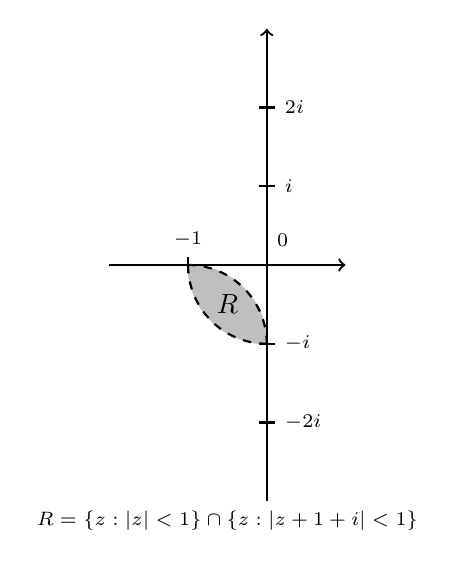
\begin{tikzpicture}
	% shading - must be drawn before the rest!
	\filldraw[color=lightgray] (-1,0) arc (0:90:-1) (0,-1) arc (0:90:1);
	\draw (-0.5,-0.5) node {$R$};
	% grid for draft only
	%%\draw [help lines] (-2,-3) grid (1,3);
	% legend
	\draw (-0.5,-3) node[below] {\scriptsize $R=\{z:|z|<1\} \cap \{z:|z+1+i|<1\}$};
	% the X-axis
	\draw[->,thick] (-2,0)--(1,0);
	\draw[thick] (-1,-0.1) -- (-1,0.1) node[above] {\scriptsize $-1$};
	\draw[thick] ( 0,-0.1) -- ( 0,0.1) node[above right] {\scriptsize $0$};
	% the Y-axis
	\draw[->,thick] (0,-3)--(0,3);
	\draw[thick] (-0.1,-1) -- (0.1,-1) node[right] {\scriptsize $-i$};
	\draw[thick] (-0.1,-2) -- (0.1,-2) node[right] {\scriptsize $-2i$};
	\draw[thick] (-0.1, 1) -- (0.1, 1) node[right] {\scriptsize $ i$};
	\draw[thick] (-0.1, 2) -- (0.1, 2) node[right] {\scriptsize $ 2i$};
	% inner circle border
	\draw[thick,style=dashed] (-1,0) arc (0:90:-1);
	% outer circle border
	\draw[thick,style=dashed] (0,-1) arc (0:90:1);
\end{tikzpicture}
%%\bigskip
%
%	The Region S
%
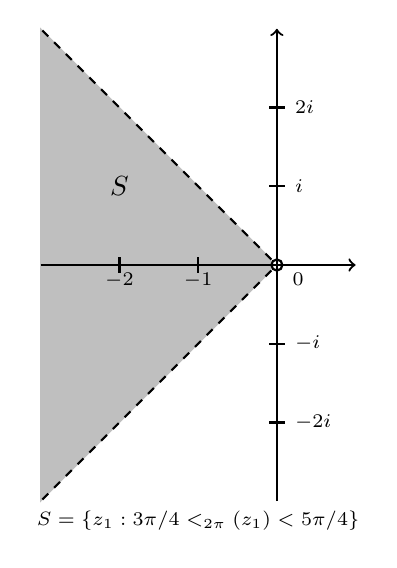
\begin{tikzpicture}
	% shading - must be drawn before the rest!
	\filldraw[color=lightgray] (-2pt,2pt) -- (-3,3) -- (-3,-3) -- (-2pt,-2pt);
	\draw (-2,1) node {$S$};
	% grid for draft only
	%%\draw [help lines] (-3,-3) grid (1,3);
	% legend
	\draw (-1,-3) node[below]
		{\scriptsize $S=\{z_1: 3\pi/4 < \Arg_{2\pi}(z_1) < 5\pi/4 \}$};
	% the X-axis
	\draw[->,thick] (-3,0)--(1,0);
	\draw[thick] (-2,-0.1) -- (-2,0.1) node[below=2pt] {\scriptsize $-2$};
	\draw[thick] (-1,-0.1) -- (-1,0.1) node[below=2pt] {\scriptsize $-1$};
	\draw[thick] ( 0,-0.1) -- ( 0,0.1) node[below right=2pt] {\scriptsize $0$};
	% the Y-axis
	\draw[->,thick] (0,-3)--(0,3);
	\draw[thick] (-0.1,-1) -- (0.1,-1) node[right] {\scriptsize $-i$};
	\draw[thick] (-0.1,-2) -- (0.1,-2) node[right] {\scriptsize $-2i$};
	\draw[thick] (-0.1, 1) -- (0.1, 1) node[right] {\scriptsize $ i$};
	\draw[thick] (-0.1, 2) -- (0.1, 2) node[right] {\scriptsize $ 2i$};
	% upper ray
	\draw[thick,style=dashed] (-2pt, 2pt) -- (-3,3);
	% lower ray
	\draw[thick,style=dashed] (-2pt,-2pt) -- (-3,-3);
	% exclude the origin
	\draw[thick] (0,0) circle(2pt);
\end{tikzpicture}

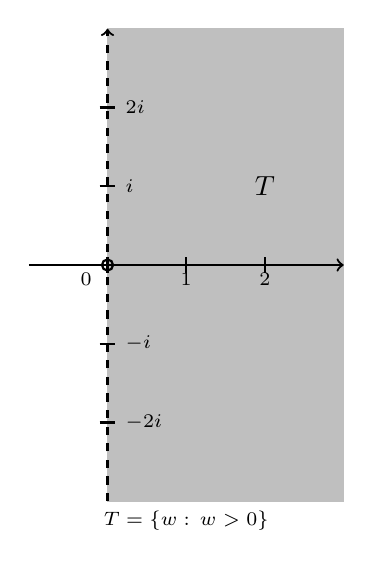
\begin{tikzpicture}
	% shading - must be drawn before the rest!
	\filldraw[color=lightgray] (0,3) -- (3,3) -- (3,-3) -- (0,-3) -- cycle;
	\draw (2,1) node {$T$};
	% grid for draft only
	%%\draw [help lines] (-1,-3) grid (3,3);
	% legend
	\draw (1,-3) node[below]
		{\scriptsize $T=\{ w: \RE\,w > 0 \} $};
	% the X-axis
	\draw[->,thick] (-1,0)--(3,0);
	\draw[thick] ( 2,-0.1) -- ( 2,0.1) node[below=2pt] {\scriptsize $ 2$};
	\draw[thick] ( 1,-0.1) -- ( 1,0.1) node[below=2pt] {\scriptsize $ 1$};
	\draw[thick] ( 0,-0.1) -- ( 0,0.1) node[below left=2pt] {\scriptsize $0$};
	% the Y-axis
	\draw[->,thick,style=dashed] (0,-3)--(0,3);
	\draw[thick] (-0.1,-1) -- (0.1,-1) node[right] {\scriptsize $-i$};
	\draw[thick] (-0.1,-2) -- (0.1,-2) node[right] {\scriptsize $-2i$};
	\draw[thick] (-0.1, 1) -- (0.1, 1) node[right] {\scriptsize $ i$};
	\draw[thick] (-0.1, 2) -- (0.1, 2) node[right] {\scriptsize $ 2i$};
	% exclude the origin
	\draw[thick] (0,0) circle(2pt);
\end{tikzpicture}


\item[(ii)]

The two boundaries (arcs) on $R$ map to the two boundaries (rays) in $S$.

$R$ is bounded, and $-i$ on $R$ is mapped to $\infty$ on $S$, which
is unbounded.

The angle of intersection of the arcs on $R$ at $-1$ is $\frac{\pi}{2}$,
this angle is preserved on the intersection of the two boundary rays of
$S$ at $0$.

The point $\infty$ is outside the bounded region $R$, this point is
mapped to $1$, which is also outside $S$

The point $\frac{1}{2}(-1-i)$ is in $R$, this point maps to $-1$, which
is in $S$.

Hence, $f$ is a conformal mapping from $R$ to $S$.

\item[(iii)]

We can map the region $S$ to the region $T$ with the square function,
$f_2(z_1)=z_1^2$, so $z_1\in S$ is mapped to $w\in T$.

Since the M\"{o}bius Transformation, $f_1$, is one-one and conformal
on $R$ and the square function, $f_2$, is one-one and conformal on $S$,
we can use their composite to map $R$ to $T$, $f = f_2 \circ f_1$, hence
\[
f(z) = f_2 ( f_1(z) ) = \left( \frac{ z+1 }{ z+i } \right)^2
\]
is a one-one conformal mapping from $R$ to $T$.

\item[(iv)]
For the inverse function we have $f^{-1} = f_1^{-1} \circ f_2^{-1}$,
where
\[
z_1 = f_2^{-1}(w) = -\sqrt{w}
\]
and\hbm{D1}{2.6}
\[
z = f_1^{-1}(z_1) = \frac{ iz_1 - 1 }{ -z_1 + 1 }
\]
Hence,
\[
z	= f^{-1}(w)
	= \frac{ i(-\sqrt{w}) - 1 }{ -(-\sqrt{w}) + 1 }
	= \frac{ -i\sqrt{w} - 1 }{ \sqrt{w} + 1 }
\]

\end{itemize}

\end{itemize}

